\section{On a serial task, a loop buys extendable depth}
\label{sec:serial}

To test the second claim where iterating should matter, we built the chain task, a task that needs serial steps, and
froze its design, conditions and predictions before its main runs; it uses the same architecture as the language
models. Pilot runs then led to three changes before any formal run, all to make the task
learnable: the operations became lookup tables instead of modular arithmetic, a curriculum was added, and training was
lengthened. The last of these came after a one-seed pilot of all conditions, and the
learning-rate protocol was fixed after that (Appendix~\ref{app:deviations}).

\subsection{The task and the conditions}
\label{sec:task}

A problem lists a start value and a sequence of table lookups (Figure~\ref{fig:schematic}b), for example
\texttt{25 ; LUT 7 ; LUT 3 ; LUT 19 ; \ldots\ =>} after a start marker. Here \texttt{LUT k} means ``look up the
current value in table $T_k$'', one of 32 fixed random tables that map $\{0,\ldots,96\}$ to itself. Each lookup is one
step: the $j$-th gives the intermediate value $x_j$, and a chain of $d$ steps has $d$ lookups and a prompt of $3d + 4$
tokens. The model must output the final value in a single forward pass, and the loss is taken at the answer position
only. Two consecutive lookups can form any of the $32 \times 32 = 1024$ compositions of two tables, so a model that
skips steps must memorise tables of compositions, which grow rapidly with the number of steps skipped. Because
composition is associative, the chain could in principle be computed in fewer serial steps than it has lookups
\citep{liu2022shortcuts}.

Models are trained on chains of 1--8 steps for 32{,}000 training steps, with batches of 512 problems sampled online and
a curriculum that widens the range of lengths over the first half of training. They are tested on 2{,}000 newly drawn
problems at every length from 1 to 24. Chains longer than 8 steps never occur in training, but short ones repeat: every
test problem with 1 or 2 steps, and about half of those with 3, also occurs in training (there are only 3{,}104
one-step problems).

All models have width 256. The dense models have 8, 20 or 36 layers (6.5M, 16.1M and 29.0M parameters); those with 20
and 36 layers match the executed depth of the looped models with 4 and 8 loops. The looped models have 8 layers (6.6M
parameters), with a middle block of four layers looped $r$ times. They are trained with $r = 2$, 4 or 8 loops, with a
random loop count drawn from 1--8 at every training step, or with as many loops as the chain has steps (``loops =
steps'', the regime of \citealp{fan2025looped}). A fourth regime, loops = steps with a few random extra loops (S9), is
introduced in Section~\ref{sec:stopping}. In S5 (\lbl{pre-specified}), dense models write the values of the chain out
as tokens, the last of them the answer. This chain of thought \citep{wei2022chain} is trained from scratch on the
written values, as in scratchpad training \citep{nye2021show}, with 8 layers (the looped models' size) and with 36 (the
8-loop model's executed depth). We also train an 8-layer dense model given $d$ pause tokens before the answer
\citep{goyal2024think}.

Every condition has five seeds, and its learning rate was chosen by a sweep on in-range accuracy only. The looped
models' rates came out 4--8 times lower than that of the 8-layer dense model, which has the same unique layers
(Appendix~\ref{app:synthetic}). The design fixed five predictions (P1--P5, Section~\ref{sec:predictions}). A planned
control task, pointer chasing, was not learned by any condition tried on it and was dropped
(Appendix~\ref{app:synthetic}).

\subsection{Within the training range, a loop adds depth, and a written chain of thought does so more cheaply}
\label{sec:inrange}

At equal parameters, the largest solvable length rises with the number of loops: from 4.2 steps for the 8-layer dense
model to 6.4, 8.0 and 9.0 steps with 2, 4 and 8 loops (seed means; Table~\ref{tab:chain}, \lbl{pre-specified}). Within
the training range, the 8-loop model is at 0.998 where the 8-layer dense model is at 0.62.

\begin{table}[t]
  \centering
  \caption{The chain task, trained on 1--8 steps (seed means; chance is 0.01; accuracies rounded, and only the
  chain-of-thought models are exactly perfect in range). \emph{Largest solvable length}: the longest chain length up to
  which every length is solved with accuracy $\geq 0.9$ (mean, and min--max over five seeds). The frozen design's measure, the largest length solved at $\geq 0.9$ without requiring every shorter length, gives the
  same values in the \emph{Training loops} column and differs only for 2 loops under \emph{More loops} (10.4 instead of
  8.6). \emph{Training loops}: at the training loop count (8 for the random loop count, $d$ for loops = steps; dense
  models as trained). \emph{More loops}: the training loop count or any larger count tried, including $d$ loops,
  whichever is best for each seed, chosen using the test answers (a reference, not a rule a model could apply); the set
  of counts was widened after the results (Appendix~\ref{app:deviations}). ``---'': not applicable. \emph{Layer passes}:
  executed layers times tokens processed for a 12-step problem, that is, a prompt of 40 tokens, plus the 11 written values that precede the answer for the
  chain-of-thought models (each fed back with a KV cache; the answer itself is not processed) or 12 pause tokens.}
  \label{tab:chain}
  \footnotesize
  \setlength{\tabcolsep}{2.6pt}
  \begin{tabular}{lccccccc}
    \toprule
    & & & Within the range & \multicolumn{2}{c}{Largest solvable length} & \multicolumn{2}{c}{Beyond the range} \\
    \cmidrule(lr){4-4}\cmidrule(lr){5-6}\cmidrule(lr){7-8}
    & & Layer & Acc. & Training & More & Acc.\ 12 steps & Acc.\ 16 steps \\
    Model & Params & passes & 1--8 steps & loops & loops & train.\ / more & train.\ / more \\
    \midrule
    \multicolumn{8}{l}{\emph{Equal parameters}} \\
    Dense, 8 layers               & 6.5M & 320  & 0.621 & 4.2 (4--5)   & ---           & 0.06        & 0.05        \\
    Looped, $r=2$                 & 6.6M & 480  & 0.906 & 6.4 (6--7)   & 8.6 (6--11)   & 0.05 / 0.64 & 0.04 / 0.33 \\
    Looped, $r=4$                 & 6.6M & 800  & 1.000 & 8.0 (8--8)   & 11.8 (10--15) & 0.03 / 0.83 & 0.03 / 0.28 \\
    Looped, $r=8$                 & 6.6M & 1440 & 0.998 & 9.0 (9--9)   & 11.2 (11--12) & 0.04 / 0.86 & 0.03 / 0.37 \\
    Looped, random loop count     & 6.6M & 1440 & 0.999 & 11.4 (10--13) & 12.2 (10--15) & 0.77 / 0.83 & 0.08 / 0.49 \\
    Looped, loops = steps         & 6.6M & 2080 & 1.000 & 12.8 (11--16) & 12.8 (11--16) & 0.96 / 0.96 & 0.37 / 0.37 \\
    Loops = steps + 0--4 extra (S9) & 6.6M & 2080 & 0.999 & 11.6 (11--12) & 12.2 (12--13) & 0.90 / 0.94 & 0.31 / 0.48 \\
    \midrule
    \multicolumn{8}{l}{\emph{Equal executed depth, which here is equal compute}} \\
    Dense, 20 layers (as $r=4$)   & 16.1M & 800  & 0.910 & 6.4 (6--7)  & ---           & 0.04        & 0.03        \\
    Dense, 36 layers (as $r=8$)   & 29.0M & 1440 & 0.999 & 8.0 (8--8)  & ---           & 0.02        & 0.02        \\
    \midrule
    \multicolumn{8}{l}{\emph{Dense models with written-out reasoning or pause tokens (S5)}} \\
    Chain of thought, 8 layers   & 6.5M  & 408  & 1.000 & 8.0 (8--8) & ---          & 0.01        & 0.01        \\
    Chain of thought, 36 layers  & 29.0M & 1836 & 1.000 & 8.0 (8--8) & ---          & 0.02        & 0.01        \\
    $d$ pause tokens, 8 layers   & 6.5M  & 416  & 0.566 & 4.0 (4--4) & ---          & 0.01        & 0.01        \\
    \bottomrule
  \end{tabular}
\end{table}

At equal executed depth, and so at equal compute, the looped models are at least as good as the dense ones. A dense
model of equal executed depth has the same width as the looped model and is trained for the same number of training
steps on the same problems. On this task it therefore costs about the same training and inference compute, but it has
2.4--4.4 times the parameters, and if the extra parameters matter, they help the dense model. The 20-layer dense model
solves 6.4 steps against 8.0 for 4 loops, though it did not fully learn the training range (0.91). Its learning rate
was chosen in a sweep whose runs were half as long as the formal runs, and in that sweep it reached 0.98
(Appendix~\ref{app:synthetic}). The 36-layer dense model solves 8.0 steps against 9.0 for 8 loops, and the two are
level within the range. These lengths are the plan's measure, the solvable length at the training loop count;
Section~\ref{sec:extension} discusses the \emph{More loops} columns.

On text, the dense model of equal compute has the looped model's size and more data. Here it has more parameters and
the same data, and it does not beat the loop. We do not take these two comparisons as evidence that the loop saves
compute, since one dense model did not fully learn the range and the other is level with the loop within it.

A written chain of thought is perfect within the training range and costs less than the loop. It scores 1.000 in every
seed and at every learning rate tried, where the 8-layer model that answers directly solves 4 steps. At any length it
needs under a third of the inference compute of the 8-loop model: 408 against 1440 layer passes at 12 steps
(Table~\ref{tab:chain}). The comparison favours it, because it is trained with a loss on every intermediate value and
the other models on the answer only. The plan stated this difference in advance, and a looped model with intermediate
supervision was outside it. Pause tokens add nothing: the pause model solves the same 4 steps as the model without
them.

\begin{figure}[t]
  \centering
  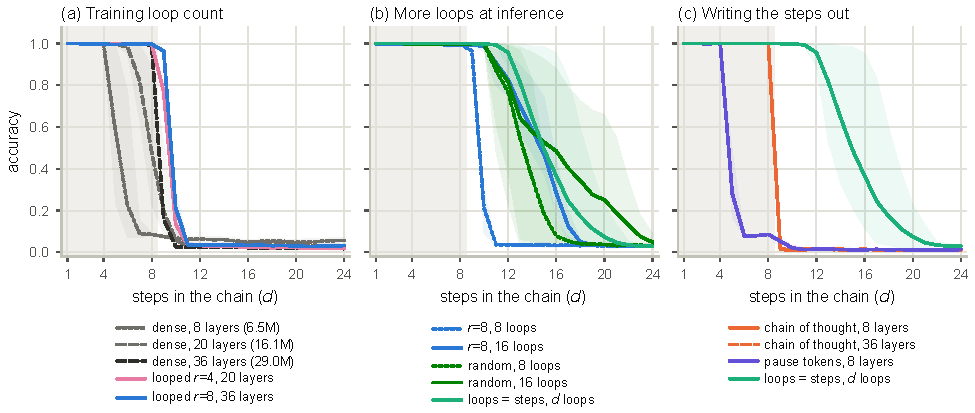
\includegraphics[width=\linewidth]{fig5_chain}
  \caption{The chain task, trained on 1--8 steps (shaded): accuracy against chain length, mean over five seeds (band:
  range). \textbf{(a)}~At the training loop count, looped models solve at least as far as dense models of the same
  executed depth, and none gets more than one step past the training range. \textbf{(b)}~With more loops at inference,
  the looped models solve longer chains; the model trained with as many loops as steps, run with $d$ loops, solves the
  longest chains at accuracy 0.9. \textbf{(c)}~Dense models that write the chain out are perfect within the training
  range and near chance beyond it; pause tokens add nothing (the loops = steps model is replotted for comparison).}
  \label{fig:chain}
\end{figure}

\subsection{Beyond the training range, only the loop extends}
\label{sec:extension}

We say that a model \emph{extends} if, given more computation at inference, it solves chains longer than those it was
trained on. At their training loop count, neither the dense models nor the fixed-loop models get more than one step
past the training range: at 12 steps, the dense models that answer directly score 0.01--0.06 and the fixed-loop models
0.03--0.05 (Figure~\ref{fig:chain}a).

Run with more loops, the looped models extend (Figure~\ref{fig:chain}b). The model trained with 8 loops solves 9 steps
at 8 loops and about 11 with 16 or 32. At 12 steps its accuracy rises from 0.04 to 0.83 at 16 loops, and to 0.86 when
the best loop count between 12 and 32 is chosen for each seed using the answers (seed means). The gain is limited,
though: at 16 steps the best is 0.37, with a wide spread across seeds. The model trained with a random loop count gains
as well (0.08 to 0.49 at 16 steps), against the frozen prediction that it would not. Run with as many loops as the
chain has steps, the loops = steps model solves the longest chains at accuracy 0.9 (12.8 steps). Part of this comes
from being told how long to run, since its loop count is the number of steps, which the prompt shows. With $d$ loops it
is 0.34--0.95 more accurate than with 8 at every length from 10 to 16 (we count from 10 steps, a choice made after the
results; at 9 steps the difference is 0.03).

The written chain of thought, perfect within the training range (Section~\ref{sec:inrange}), does not extend at all.
It scores 0.014 at 12 steps with 8 layers and 0.017 with 36, near the chance level of 0.010, on prompts on which the
looped models trained with 4 or more loops reach 0.83--0.96 (Figure~\ref{fig:chain}c). S5 had predicted at least 0.7
for the 8-layer model and at least 0.8 for the 36-layer one. The 8-layer model breaks at the start. On problems with
more than 8 steps, its first wrong token is one of the first three written ones in 97--98\% of the problems
\lbl{(exploratory)}, so its errors do not build up along the chain. Because the prompt of this task grows with the
number of steps, the chain of thought may be failing to generalise to longer inputs, a known weakness of transformers
\citep{zhou2024transformers,cho2024position}, rather than to more steps. The comparison cannot say whether a written
chain would extend on a task whose input length does not grow; we did not run such a task, and remedies for length
generalisation were outside the plan. Pause tokens do not extend either, as S5 predicted.

\subsection{The loop computes the chain step by step}
\label{sec:probes}

For each intermediate value $x_j$, we trained a linear probe on the state after every loop, on problems with 8 steps
and with the looped models running 16 loops (Figure~\ref{fig:probes}). The probes were planned in the frozen design;
the summaries below are \lbl{exploratory}. Each probe reads three prompt positions around step $j$ (its table number,
the separator after it and the next lookup token), and the best of the three counts.

With a loop for every step, the chain advances one step per loop. In the model trained with 8 loops, $x_j$ first
becomes decodable (probe accuracy $\geq 0.5$) at about loop $j$, at 1.0--1.1 loops per step in all five seeds. It
stays decodable afterwards, with a lowest probe accuracy at later loops of 0.96, averaged over the values. The loops =
steps model also computes one step per loop and keeps its values for its $d$ loops (lowest later accuracy 0.92), but
it loses them when run longer. It was never trained to keep looping after the last step, which is why it needs exactly
$d$ loops.

Models with fewer loops than steps pack several steps into each loop, about 1.6 with 4 loops and 2.4 with 2, in the
direction that \citet{zhang2026recurrence} predict. In these models the last values become decodable at the step
positions only after the training loop count: at loop 5 with 4 loops, and at loops 3--4 with 2.

The dense models compute the values late, from about layer 21 of 36, and in 5 of the 10 dense seeds (five at 20 layers
and five at 36) no intermediate value after $x_1$ is decodable. These probes are consistent with the extension results:
a loop that applies the same step each time can be run for more steps, while a stack that computes the chain in its
last layers cannot. A probe shows where a value can be read out; it does not show that the model uses the value.

\begin{figure}[t]
  \centering
  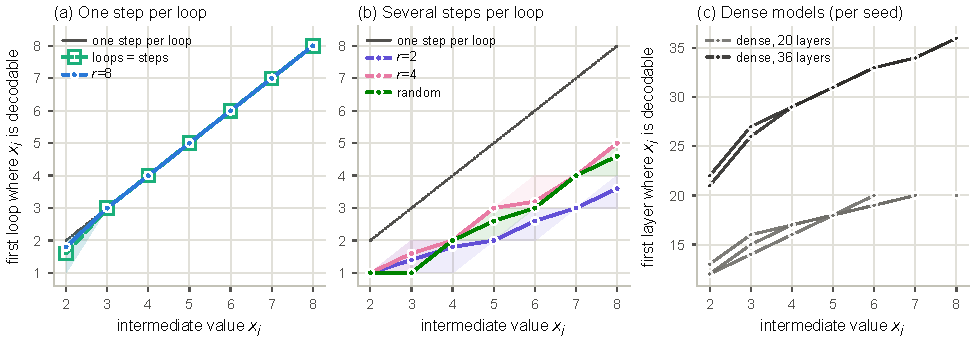
\includegraphics[width=\linewidth]{fig6_chain_probes}
  \caption{Where the intermediate values appear (probes on 8-step problems; a value counts as decodable at probe
  accuracy $\geq 0.5$). \textbf{(a)}~With a loop for every step, the chain advances one step per loop. \textbf{(b)}~With
  fewer loops than steps, each loop advances several steps (mean over seeds; band: range; looped models probed while
  running 16 loops). \textbf{(c)}~Dense models compute the values late in their depth (one line per seed). A seed in
  which only $x_1$, not plotted, and the answer are decodable appears as a single point at the last layer; the 20-layer
  seed with no decodable intermediate value is not shown.}
  \label{fig:probes}
\end{figure}

\subsection{The learning rate decides whether the loop learns the task within 32{,}000 training steps}
\label{sec:lrsynthetic}

At $10^{-3}$, a good rate for the dense models, the 8-loop model of the learning-rate sweep worked only at its training
count of 8 loops and at no other count from 2 to 32, like the language models of Section~\ref{sec:mechanism}. No
intermediate value became decodable one loop per step. But it had also learned the training range much worse: 0.54,
against 0.999 at $2.5\times10^{-4}$.

A supplementary experiment (S2, \lbl{pre-specified}) asked whether a high rate changes what the looped model learns or
how fast it learns. It trained the four looped conditions named in its plan ($r = 4$, $r = 8$, the random loop count
and loops = steps) for 32{,}000 training steps with three seeds. At $10^{-3}$ they did not learn the training range in
10 of 12 runs; at $5\times10^{-4}$ they learned it in 8 of 12, and those runs mostly extended about as far as the formal
runs (Appendix~\ref{app:synthetic}). A high learning rate mainly keeps the looped model from learning the task within
the given training steps, and when the model does learn the task, it mostly learns the same extendable algorithm. By
the plan's own criteria, the learning rate changed the solution in one of the eight combinations of condition and
rate, the random loop count at $5\times10^{-4}$ (Appendix~\ref{app:synthetic}).

\subsection{Stopping without the answer}
\label{sec:stopping}

Most looped models can decide when to stop from their own confidence, without knowing the answer
(Table~\ref{tab:stopping}), although we chose this rule after comparing several. Extra loops help in deployment only if
their number can be set without the answer. Always running a fixed number of
extra loops works for the 8-loop model (Section~\ref{sec:extension}) but not for the loops = steps model, which loses
its values when run longer (Section~\ref{sec:probes}). The alternative is a rule that decides for each problem when to
stop.

The frozen design specified one such rule, for the loops = steps model: stop when the state changes by less than a
threshold between loops. At the freeze it was implemented as a relative change below 2\% at the answer position, with
at most 32 loops. A supplementary experiment (S8, \lbl{pre-specified}), planned after this rule's results were known
and frozen before the comparison, tested it against three other kinds of rule on the 25 checkpoints of the formal runs
(five looped conditions, five seeds each). The prediction rule stops when the predicted answer has not changed for $m$
loops, the confidence rule when the model's top probability reaches a threshold, and the vote takes the majority answer
over several loop counts. The confidence rule is an early-stopping variant of the maximum-confidence rule of
\citet{fan2025looped}, who mention this variant but do not evaluate it. All rules were fixed in the plan, selected on
one problem set and reported on another, drawn independently (Table~\ref{tab:stopping}).

\begin{table}[t]
  \centering
  \caption{Stopping without the answer: accuracy on 12-step chains (seed means, reporting set). In parentheses: mean
  loops used, where given; Table~\ref{tab:s8} gives them for every rule. The best fixed loop count is chosen with the
  answers; it is a reference, not a rule, and an adaptive rule can exceed it ($r = 2$).}
  \label{tab:stopping}
  \footnotesize
  \begin{tabular}{l>{\centering\arraybackslash}p{0.08\linewidth}>{\centering\arraybackslash}p{0.08\linewidth}>{\centering\arraybackslash}p{0.09\linewidth}>{\centering\arraybackslash}p{0.11\linewidth}>{\centering\arraybackslash}p{0.22\linewidth}}
    \toprule
    Model & Training loop count & Best fixed count & State change $<2\%$ & State change $<0.5\%$ & Confidence $\geq 0.99$ \\
    \midrule
    Looped, $r=2$ & 0.05 & 0.62 & 0.45 & 0.45 (32) & 0.70 (8.3) \\
    Looped, $r=4$ & 0.04 & 0.83 & 0.65 & 0.82 (27) & 0.81 (9.2) \\
    Looped, $r=8$ & 0.04 & 0.86 & 0.71 & 0.84 (28) & 0.84 (17) \\
    Random loop count & 0.77 & 0.83 & 0.73 & 0.83 (22) & 0.83 (14) \\
    Loops = steps ($d$ loops) & 0.96 & 0.96 & 0.03 & 0.03 (29) & 0.76 (14)$^{a}$ \\
    Loops = steps + 0--4 extra (S9) & 0.90 & 0.94 & 0.52 & 0.94 (24) & 0.93 (14)$^{b}$ \\
    \bottomrule
    \multicolumn{6}{l}{\footnotesize $^{a}$\,6--7\% of the in-range problems lost; $^{b}$\,0.998 of the in-range problems kept.} \\
  \end{tabular}
\end{table}

The frozen state rule recovers about 80\% of the gain of the best fixed loop count at 12 steps for the models trained
with 4 or 8 loops, without hurting the training range. It cannot stop the loops = steps model, whose state keeps
changing after $d$ loops (accuracy 0.02--0.08 at every length).

The confidence rule does better. At a threshold of 0.99 it recovers 97--98\% of that gain for the models trained with 4
or 8 loops or a random count, and on in-range problems it uses fewer loops than their training count. It brings the
loops = steps model to 0.76, but loses 6--7\% of the in-range problems. Among the rules that stop, a confidence rule (at
0.99, or at 0.9 for $r = 2$) is the best, or within 0.001 of it, in every condition of S8. A state rule with a lower
threshold (0.5\%) comes within 0.005 of the confidence rule for 4 and 8 loops and the random loop count, and for $r = 4$
is slightly above it (0.816 against 0.815). But it uses 1.5 to 3 times as many loops. The prediction rule often stops on
a wrong answer that no longer changes, and the votes run all 32 loops and never beat the best fixed count.

We singled out the confidence rule only after this comparison. The selection criterion of the S8 plan picked a vote for
three of the five conditions, and with votes set aside it picked the confidence rule at 0.99 only for $r = 8$ and the
random loop count (Appendix~\ref{app:synthetic}). Two of the plan's five predictions held: the prediction rule stayed
within 1.5 times the training loop count on in-range problems, and the votes did not beat the best fixed count.
Contrary to the plan, the prediction rule neither beat the state rule nor recovered 85\% of the gain for $r = 4$ and
$r = 8$, and the confidence rule took the loops = steps model above the predicted ceiling of 0.2.

The models that extend furthest and the models that stop well came from different training regimes. A supplementary
experiment (S9, \lbl{pre-specified}) trained the loops = steps model with 0--4 random extra loops after the last step.
The resulting model keeps its values when run longer (lowest probe accuracy over 16 loops 0.04 $\rightarrow$ 0.91) and
extends about one step less (11.6 against 12.8). With the confidence rule it reaches 0.93 on 12-step problems
(0.89--0.95 in the five seeds) while still solving 0.998 of the problems within the training range. So a few extra
loops in training give a model that both extends and stops. The 0.5\% state rule is slightly better (0.94 against
0.93, and better in all five seeds), but runs 24 loops against 14. With the frozen state rule, how well the model stops
depends on the seed: the rule works in two seeds, fails in two and partly works in the fifth, for a mean of 0.52 at 12
steps. The plan had predicted at least 0.6, and this is the only one of its four predictions that failed. None of
the three outcomes the plan anticipated covers this combination of results. Training the model costs about 1.4 times
the compute per training step of the loops = steps model.

\subsection{The pre-specified predictions}
\label{sec:predictions}

The frozen design made five predictions (Table~\ref{tab:p1p5} in Appendix~\ref{app:synthetic}):
\begin{itemize}
  \item \textbf{P1}: the largest solvable length rises from the dense model through 2, 4 and 8 loops, and reaches at
  least 16 steps with 8 loops. It holds in direction, but the 8-loop model reached 9 steps.
  \item \textbf{P2}: dense models of equal executed depth are at least as good as the looped models. The looped models
  solve 1--1.6 more steps, so P2 is not supported.
      \item \textbf{P3}: three predictions about running a model with a loop count other than its training count.
  (a)~Fixed-loop models get much worse. This is half right: they get worse with fewer loops, but the 4- and 8-loop
  models do not get worse with more. (b)~The random-loop model does not gain from more loops on chains longer than 8
  steps. This fails, since the model gains (0.08 to 0.49 at 16 steps). (c)~The loops = steps model, run with $d$ loops,
  beats itself run with 8 loops at every length from 9 to at least 16. By a criterion chosen after the results, this
  holds from 10 steps on (Section~\ref{sec:extension}).
  \item \textbf{P4}: the probe table of the loops = steps model is diagonal ($x_j$ appearing at loop $j$;
  Figure~\ref{fig:probes}a), and that of the fixed-loop models is not. If a value counts as appearing at the loop where
  it first becomes decodable, a reading chosen after the results, P4 is half right, because the 8-loop model's table is
  diagonal too. Under the design's own wording, which takes the loop where a value is decoded most accurately, P4 would
  hold.
  \item \textbf{P5}: the differences between looped and dense models of equal parameters are far larger than on text.
  This holds.
\end{itemize}

On the chain task, then, the loop adds serial depth, and probes find the chain's intermediate values in its state one
after another, which is consistent with step-by-step computation. Within the training range
(Section~\ref{sec:inrange}), this depth saves no compute over a dense model of the same executed depth and costs more
than a written chain of thought. Beyond the range (Section~\ref{sec:extension}), the loop is the only form of extra
computation we tried that extends. Dense models that answer directly cannot run longer, even with the 8-loop model's
executed depth, and the chain of thought fails from its first written tokens, possibly because its prompts grow
longer than any seen in training.
